%%%%%%%%%%%%%%%%%%%%%%%%%%%%%%%%%%%%%%%%%
%
% Graduation Thesis RWJ Peelen
%
%%%%%%%%%%%%%%%%%%%%%%%%%%%%%%%%%%%%%%%%%
%----------------------------------------------------------------------------------------
%   PACKAGES AND OTHER DOCUMENT CONFIGURATIONS
%----------------------------------------------------------------------------------------

\documentclass[12pt]{Thesis}
\renewcommand{\familydefault}{\sfdefault}

\usepackage[british,UKenglish,USenglish,english,american]{babel}
\usepackage[utf8x]{inputenc}
\usepackage{graphicx}
\usepackage{wrapfig}
\usepackage{hyperref}
\usepackage[nottoc,numbib]{tocbibind}
\usepackage{url}
\usepackage{dirtytalk}
\usepackage[colorinlistoftodos]{todonotes}
\usepackage{mathtools}

\usepackage{listings}
\usepackage{color}

\usepackage{upquote}
\definecolor{editorGray}{rgb}{0.95, 0.95, 0.95}
\definecolor{editorOcher}{rgb}{1, 0.5, 0} % #FF7F00 -> rgb(239, 169, 0)
\definecolor{editorGreen}{rgb}{0, 0.5, 0} % #007C00 -> rgb(0, 124, 0)

\lstdefinelanguage{CSS}{
  morekeywords={accelerator,azimuth,background,background-attachment,
    background-color,background-image,background-position,
    background-position-x,background-position-y,background-repeat,
    behavior,border,border-bottom,border-bottom-color,
    border-bottom-style,border-bottom-width,border-collapse,
    border-color,border-left,border-left-color,border-left-style,
    border-left-width,border-right,border-right-color,
    border-right-style,border-right-width,border-spacing,
    border-style,border-top,border-top-color,border-top-style,
    border-top-width,border-width,bottom,caption-side,clear,
    clip, color,content,counter-increment,counter-reset,cue,
    cue-after,cue-before,cursor,direction,display,elevation,
    empty-cells,filter,float,font,font-family,font-size,
    font-size-adjust,font-stretch,font-style,font-variant,
    font-weight,height,ime-mode,include-source,
    layer-background-color,layer-background-image,layout-flow,
    layout-grid,layout-grid-char,layout-grid-char-spacing,
    layout-grid-line,layout-grid-mode,layout-grid-type,left,
    letter-spacing,line-break,line-height,list-style,
    list-style-image,list-style-position,list-style-type,margin,
    margin-bottom,margin-left,margin-right,margin-top,
    marker-offset,marks,max-height,max-width,min-height,
    min-width,-moz-binding,-moz-border-radius,
    -moz-border-radius-topleft,-moz-border-radius-topright,
    -moz-border-radius-bottomright,-moz-border-radius-bottomleft,
    -moz-border-top-colors,-moz-border-right-colors,
    -moz-border-bottom-colors,-moz-border-left-colors,-moz-opacity,
    -moz-outline,-moz-outline-color,-moz-outline-style,
    -moz-outline-width,-moz-user-focus,-moz-user-input,
    -moz-user-modify,-moz-user-select,orphans,outline,
    outline-color,outline-style,outline-width,overflow,
    overflow-X,overflow-Y,padding,padding-bottom,padding-left,
    padding-right,padding-top,page,page-break-after,
    page-break-before,page-break-inside,pause,pause-after,
    pause-before,pitch,pitch-range,play-during,position,quotes,
    -replace,richness,right,ruby-align,ruby-overhang,
    ruby-position,-set-link-source,size,speak,speak-header,
    speak-numeral,speak-punctuation,speech-rate,stress,
    scrollbar-arrow-color,scrollbar-base-color,
    scrollbar-dark-shadow-color,scrollbar-face-color,
    scrollbar-highlight-color,scrollbar-shadow-color,
    scrollbar-3d-light-color,scrollbar-track-color,table-layout,
    text-align,text-align-last,text-decoration,text-indent,
    text-justify,text-overflow,text-shadow,text-transform,
    text-autospace,text-kashida-space,text-underline-position,top,
    unicode-bidi,-use-link-source,vertical-align,visibility,
    voice-family,volume,white-space,widows,width,word-break,
    word-spacing,word-wrap,writing-mode,z-index,zoom},
  morestring={:}{;}[\color{red}],
  sensitive,
  morecomment=[s]{/*}{*/}
}
 
 \lstset{%
        % Basic design
        backgroundcolor=\color{editorGray},
        basicstyle={\small\ttfamily},   
        frame=l,
        % Line numbers
        xleftmargin={0.75cm},
        numbers=left,
        stepnumber=1,
        firstnumber=1,
        numberfirstline=true,
    }


\mscName{R.W.J. Peelen}%
\mscTitle{Viability of WebGL Product Configurators}%

\begin{document}

%----------------------------------------------------------------------------------------
%   TitlePage
%----------------------------------------------------------------------------------------
\begin{titlepage}

\newcommand{\HRule}{\rule{\linewidth}{0.5mm}} % Defines a new command for the horizontal lines, change thickness here

\center % Center everything on the page
 
%----------------------------------------------------------------------------------------
%   HEADING SECTIONS
%----------------------------------------------------------------------------------------

\textsc{\Large Utrecht University for Applied Sciences}\\[1cm]
\textsc{\Large Digital Communication \& Media}\\[0.5cm]
\textsc{\large Faculty for Communication \& Journalism}\\[0.5cm]

%----------------------------------------------------------------------------------------
%   TITLE SECTION
%----------------------------------------------------------------------------------------

\HRule \\[0.8cm]
{ \huge \bfseries WebGL Product Configurators}\\[1cm]
\textsc{\large Technical Viability and User Experience}\\[0.4cm]
\HRule \\[1.5cm]
 
%----------------------------------------------------------------------------------------
%   AUTHOR SECTION
%----------------------------------------------------------------------------------------

\begin{minipage}{0.4\textwidth}
\begin{flushleft} \large
\emph{Author:}\\
R.W.J. \textsc{Peelen} % Your name
\end{flushleft}
\end{minipage}
~
\begin{minipage}{0.4\textwidth}
\begin{flushright} \large
\emph{Supervisor:} \\
K. \textsc{Winkel} % Supervisor's Name
\end{flushright}
\end{minipage}\\[2cm]

% If you don't want a supervisor, uncomment the two lines below and remove the section above
%\Large \emph{Author:}\\
%John \textsc{Smith}\\[3cm] % Your name

%----------------------------------------------------------------------------------------
%   DATE SECTION
%----------------------------------------------------------------------------------------

{\large \today}\\[2cm] % Date, change the \today to a set date if you want to be precise

%----------------------------------------------------------------------------------------
%   LOGO SECTION
%----------------------------------------------------------------------------------------

% \includegraphics{logo.png}\\[1cm] % Include a department/university logo - this will require the graphicx package
 
%----------------------------------------------------------------------------------------

\vfill % Fill the rest of the page with whitespace

\end{titlepage}

%----------------------------------------------------------------------------------------
%   Abstract
%----------------------------------------------------------------------------------------
\newpage
\section{Abstract}

Peppr is a company that is specialized in building photo-realistic visualizations. Late 2014, Peppr built a product configurator for SlimFitted, a company that builds tailored shirts. They wanted their customers to be able to design their own shirts. 

Current product configurators for the web are built by splitting up the product into different layers. Every layer consists of a pack of images. In Peppr's case, there were 25 colors, 2 perspectives, 7 collars, 6 sleeves and 3 base shirts. This left Peppr with a sum of 6300 different layers (and thus, images) and when the client wants to add another color, they would have to build another set of 252 images. This is a timely and costly venture.

Peppr concluded the usual way of doing these types of projects is suboptimal and started looking for an alternative. That is where this thesis comes to play. March 2011 was the first release of WebGL (https://en.wikipedia.org/wiki/WebGL), an implementation of OpenGL technology for the web. Because WebGL renders directly from the video processor, it opens up the web to a whole new way of using 3d. The actual adoption rate has always been low because only the latest browsers would integrate the technology. Anno 2015 though, the playing field has changed. With more-and-more browsers supporting this new type of technology, the timing might be perfect to bring it to the masses.

In this thesis I will try to find if a WebGL based product configurator, is both viable in terms of technical and marketing aspects.
\newpage

%----------------------------------------------------------------------------------------
%   TOC
%----------------------------------------------------------------------------------------
\tableofcontents

%----------------------------------------------------------------------------------------
%   Introduction
%----------------------------------------------------------------------------------------
%----------------------------------------------------------------------------------------
%   Introduction
%----------------------------------------------------------------------------------------
\chapter{Introduction}

Peppr is a company that is specialised in building visualisations and animations. They were founded in 2007 and from the start, focussed on creating high-end, photorealistic imagery. They try to stay up-to-date with new technologies and are always up for a challenge. The company consists of 4 people that bind themselves using a partnership agreement.

In 2014, Peppr was asked to build a product configurator for one of their customers (SlimFitted, a company that makes tailored shirts). They wanted a platform on which their customers would be able to order customised shirts. The customer requested the configurator accommodated for 25 colors, 2 perspectives, 7 types of collars, 6 types of sleeves and 3 different plaids. The amount of possible shirt combinations was a staggering 3.150 (25 * 7 * 6 * 3) and all of those had to be rendered from two perspectives. Creating the set of images that would make this a possibility was massive. Smartly dividing the images into parts and only changing the requested image would make things a bit easier, but the overall image-set would still be huge.

Apart from the actual images needed, the end-user needs to be able to view and edit a configuration in a simple way. This means a piece of software had to be built to show the configuration to the user. In an ideal scenario, Peppr builds a piece of software that can be re-used. Unfortunately, every customer will need their own branding and every configurator may have slightly different controls. Adding to that difficulty is the image-set. It was huge to begin with, so Peppr slit it up into several parts. This meant they could change the collar while retaining the rest of the image. This was a tricky process and adding the complexity to make it re-usable would have been a massive undertaking in both time, money, resulting in a configurator that is more complex and prone to bugs.

Peppr feels there must be a better way to serve their customers in the future, so they will end up with a cheaper, more maintainable configurator. Current technologies allow the viewing of 3d models directly in the browser. In 2015, Peppr got a second request to build a configurator and started researching their possibilities. When they did, they stumbled upon a piece of technology called OpenGL (/ WebGL) and a javascript based binding to use it on the web called "three.js". This type of technology means that a 3d model can be shown directly in browser (hardware accelerated) instead of pre-rendered images. It may well be the next big thing when it comes to configurators.

A second clients order fell through, but Peppr felt the need to explore the possibilities of WebGL further nonetheless. To put it in concrete words; Is a WebGL product configurator that directly shows 3d models instead of images a viable alternative to their current workflow? Both in development, as in end user experience.







%----------------------------------------------------------------------------------------
%   Theoretical Framework
%----------------------------------------------------------------------------------------
%----------------------------------------------------------------------------------------
%   Theoretical Framework (Probleemanalyse)
%
%----------------------------------------------------------------------------------------
\chapter{Theoretical Framework}

%----------------------------------------------------------------------------------------
%   Introduction
%----------------------------------------------------------------------------------------
\section{Introduction}
To determine the difference in workload, and in-depth review of Peppr's current workflow is needed. Below is a deep-dive into the process currently used, split into a graphics and software section. A detailed outline of the 3d process will be described in the graphics section, while a peek into the software development process will be described in the software section. The split into these components will make it easier to determine possible sections of improvement later on.
Apart from the current workflow, a basic understanding of possible new technologies needs to be looked at, as well as the current market position with regards to the technologies hype-cycle and acceptance.

%----------------------------------------------------------------------------------------
%   Workflow
%----------------------------------------------------------------------------------------
\clearpage
\section{Workflows}
Peppr has done these projects and states that the usual way of building consist of two main parts. One being the images, the other, the software. In the outline below follows a brief description of how the process is currently done. 

For this thesis, we will use an example to show the differences. Please note that this process is the way Peppr handles projects like this, and, while they did try to optimise it, they in no mean imply this is the perfect way to tackle such a project. 

\say{
A chair manufacturer wants a product configurator for one of their most popular chairs. It has 25 different colour options and has 4 different subframes. Two of the subframes are steel and can be either black or plain. The other two have wooden elements and have four wood colour options.
}


%----------------------------------------------------------------------------------------
%   Graphics
%----------------------------------------------------------------------------------------
\subsection{Graphics}

%----------------------------------------------------------------------------------------
%   Image Planning
%----------------------------------------------------------------------------------------
\subsubsection{Image Planning}
Product configurators may have to deal with an exponentially growing set of options. Peppr always checks if these image sets can be split into separate components. This may make the set smaller and easier to maintain. Below is a summary of the option set, split per item so we can start calculating how many images will be necessary.
\begin{itemize}
	\item 25 colours - \textbf{(\( \alpha \))}
	\item 2 steel frames - \textbf{(\( \beta \))}
	\item 2 frame colours - \textbf{(\( \gamma \))}
	\item 2 wood frames - \textbf{(\( \delta \))}
	\item 4 wood colours - \textbf{(\( \epsilon \))}
\end{itemize}

In this case, any seat has a pick of several frame options, and several colours. But steel frames have two colours and wood frames have four colours. To calculate the full amount of options ($x$), we can use the following formula:
 
\[ f(x) = (\alpha \cdot \beta \cdot \gamma) + (\alpha \cdot \delta \cdot \epsilon)\]
\[ f(x) = (25 \cdot 2 \cdot 2) + (25 \cdot 2 \cdot 4)\]
\[ f(x) = 300\]

Going with just 1 colour more adds 12 extra renders. While this does not seem like much, these renders are built from several different files. This means an artist has to open 12 different files, and do the edit 12 times.
In some cases, you might be able to get around it using layers. In this case, splitting up the chair into a seat and frame layer will get us the following formula:

\[ f(x) = (\alpha) + (\cdot \beta \cdot \gamma) + (\cdot \delta \cdot \epsilon)\]
\[ f(x) = (25) + (2 \cdot 2) + (2 \cdot 4)\]
\[ f(x) = 37\]

This decreases the amount of renders. Unfortunately, while this works here, in some cases this is not possible. Sometimes, one of the objects is both in front and behind other objects. This makes it difficult to 'mask' and makes proper reflections tricky. Also, creating new layers does add complexity and constraints. Adding new options and layers might prove difficult when they overlap with existing layers.
\newline
Apart from difficulties in the 3d process, these layers need to be added to the software as well. Either by creating an API that serves the layers as one image (\cite{bugaboo} ), or by stacking the images client-side. The user will notice this option though, as it slows things down. This is fixed with the adoption of HTTP 2.0. This pipelines the http-requests, reducing latency (\cite{latency}).

%----------------------------------------------------------------------------------------
%   Modeling
%----------------------------------------------------------------------------------------
\subsubsection{Modeling}

\begin{wrapfigure}[12]{r}{10cm}
\vspace{-1cm}
\centering
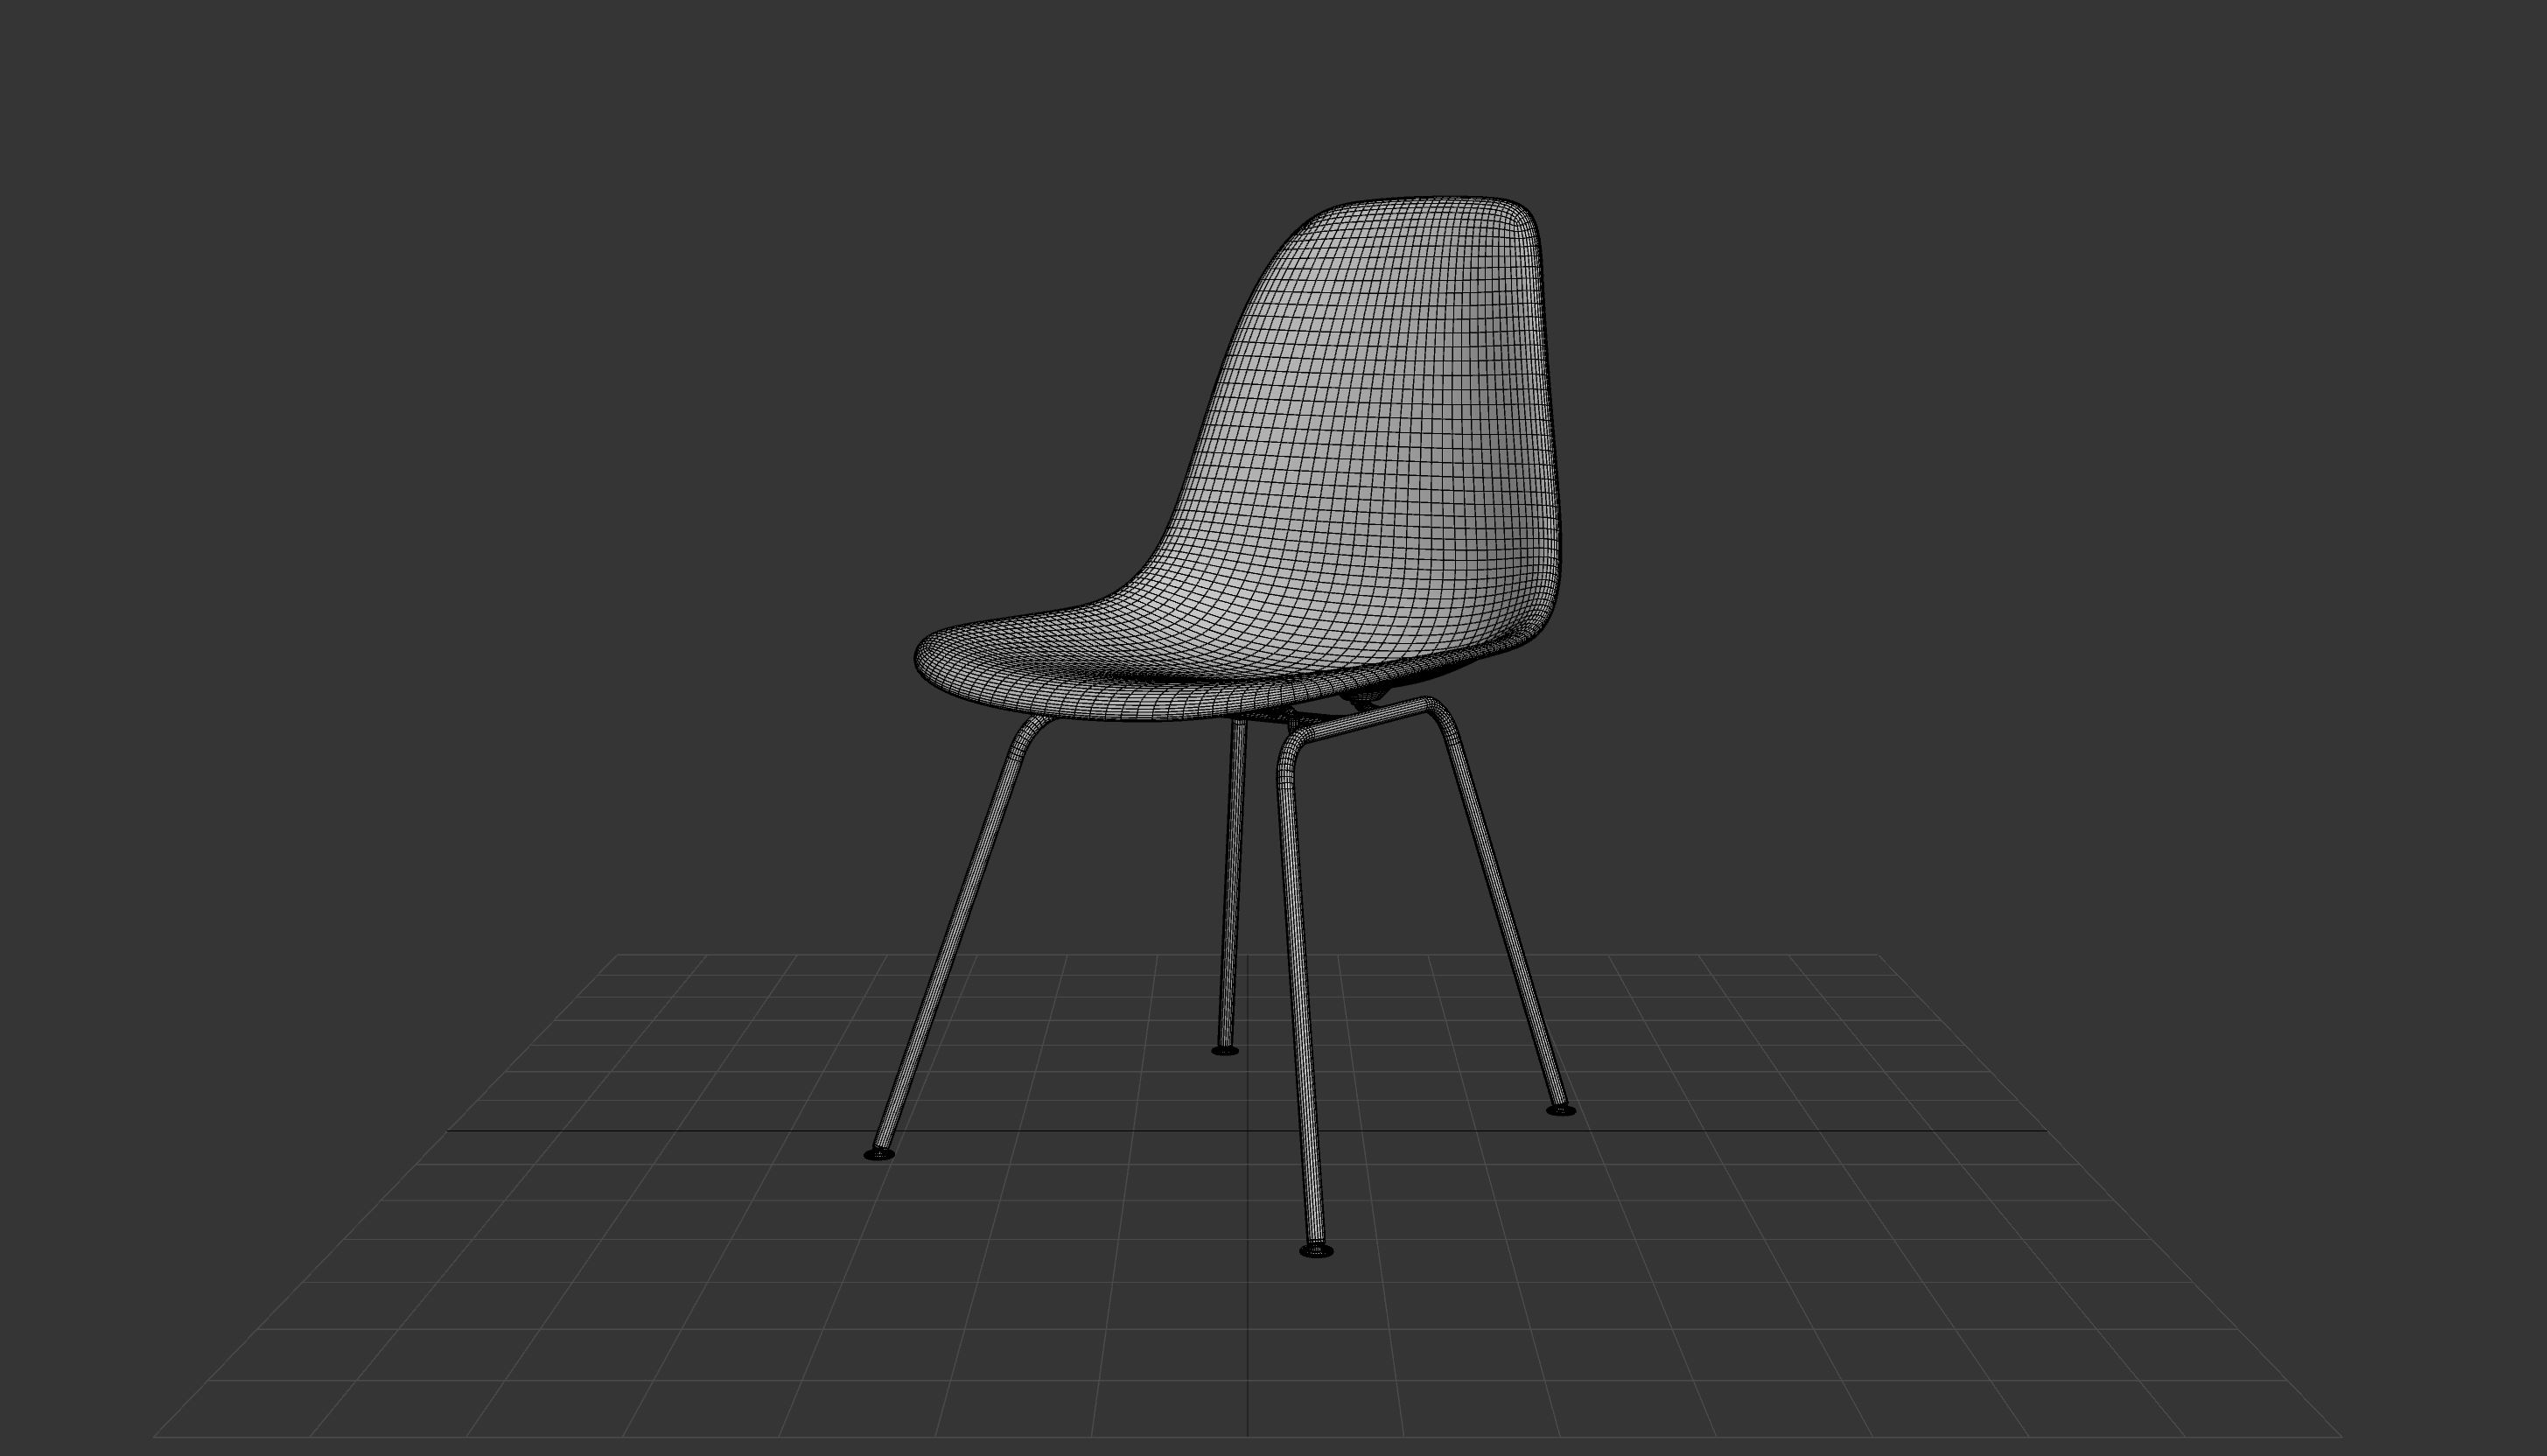
\includegraphics[width=9cm]{images/modeling}
\caption{Lighting Setup}
\label{figure:modeling}
\end{wrapfigure}


Step two in the process is modeling, whereby an artist makes a virtual model. Mostly used at Peppr is a form of modeling called Polygonal modeling. This means the model will eventually be represented by an array of 3 dimensional points (or vertices). All vertices are connected by lines and those lines make up the surface of the model. There are multiple ways of creating these models, an artist may choose to 'draw' those polygons from scratch, but may also use 3d scanning services or even simulations to build the 3d models.
As seen in \ref{figure:modeling}, every single square in that model is one of those polygons.

%----------------------------------------------------------------------------------------
%   Lighting / Shading
%----------------------------------------------------------------------------------------
\clearpage
\begin{figure}
\centering
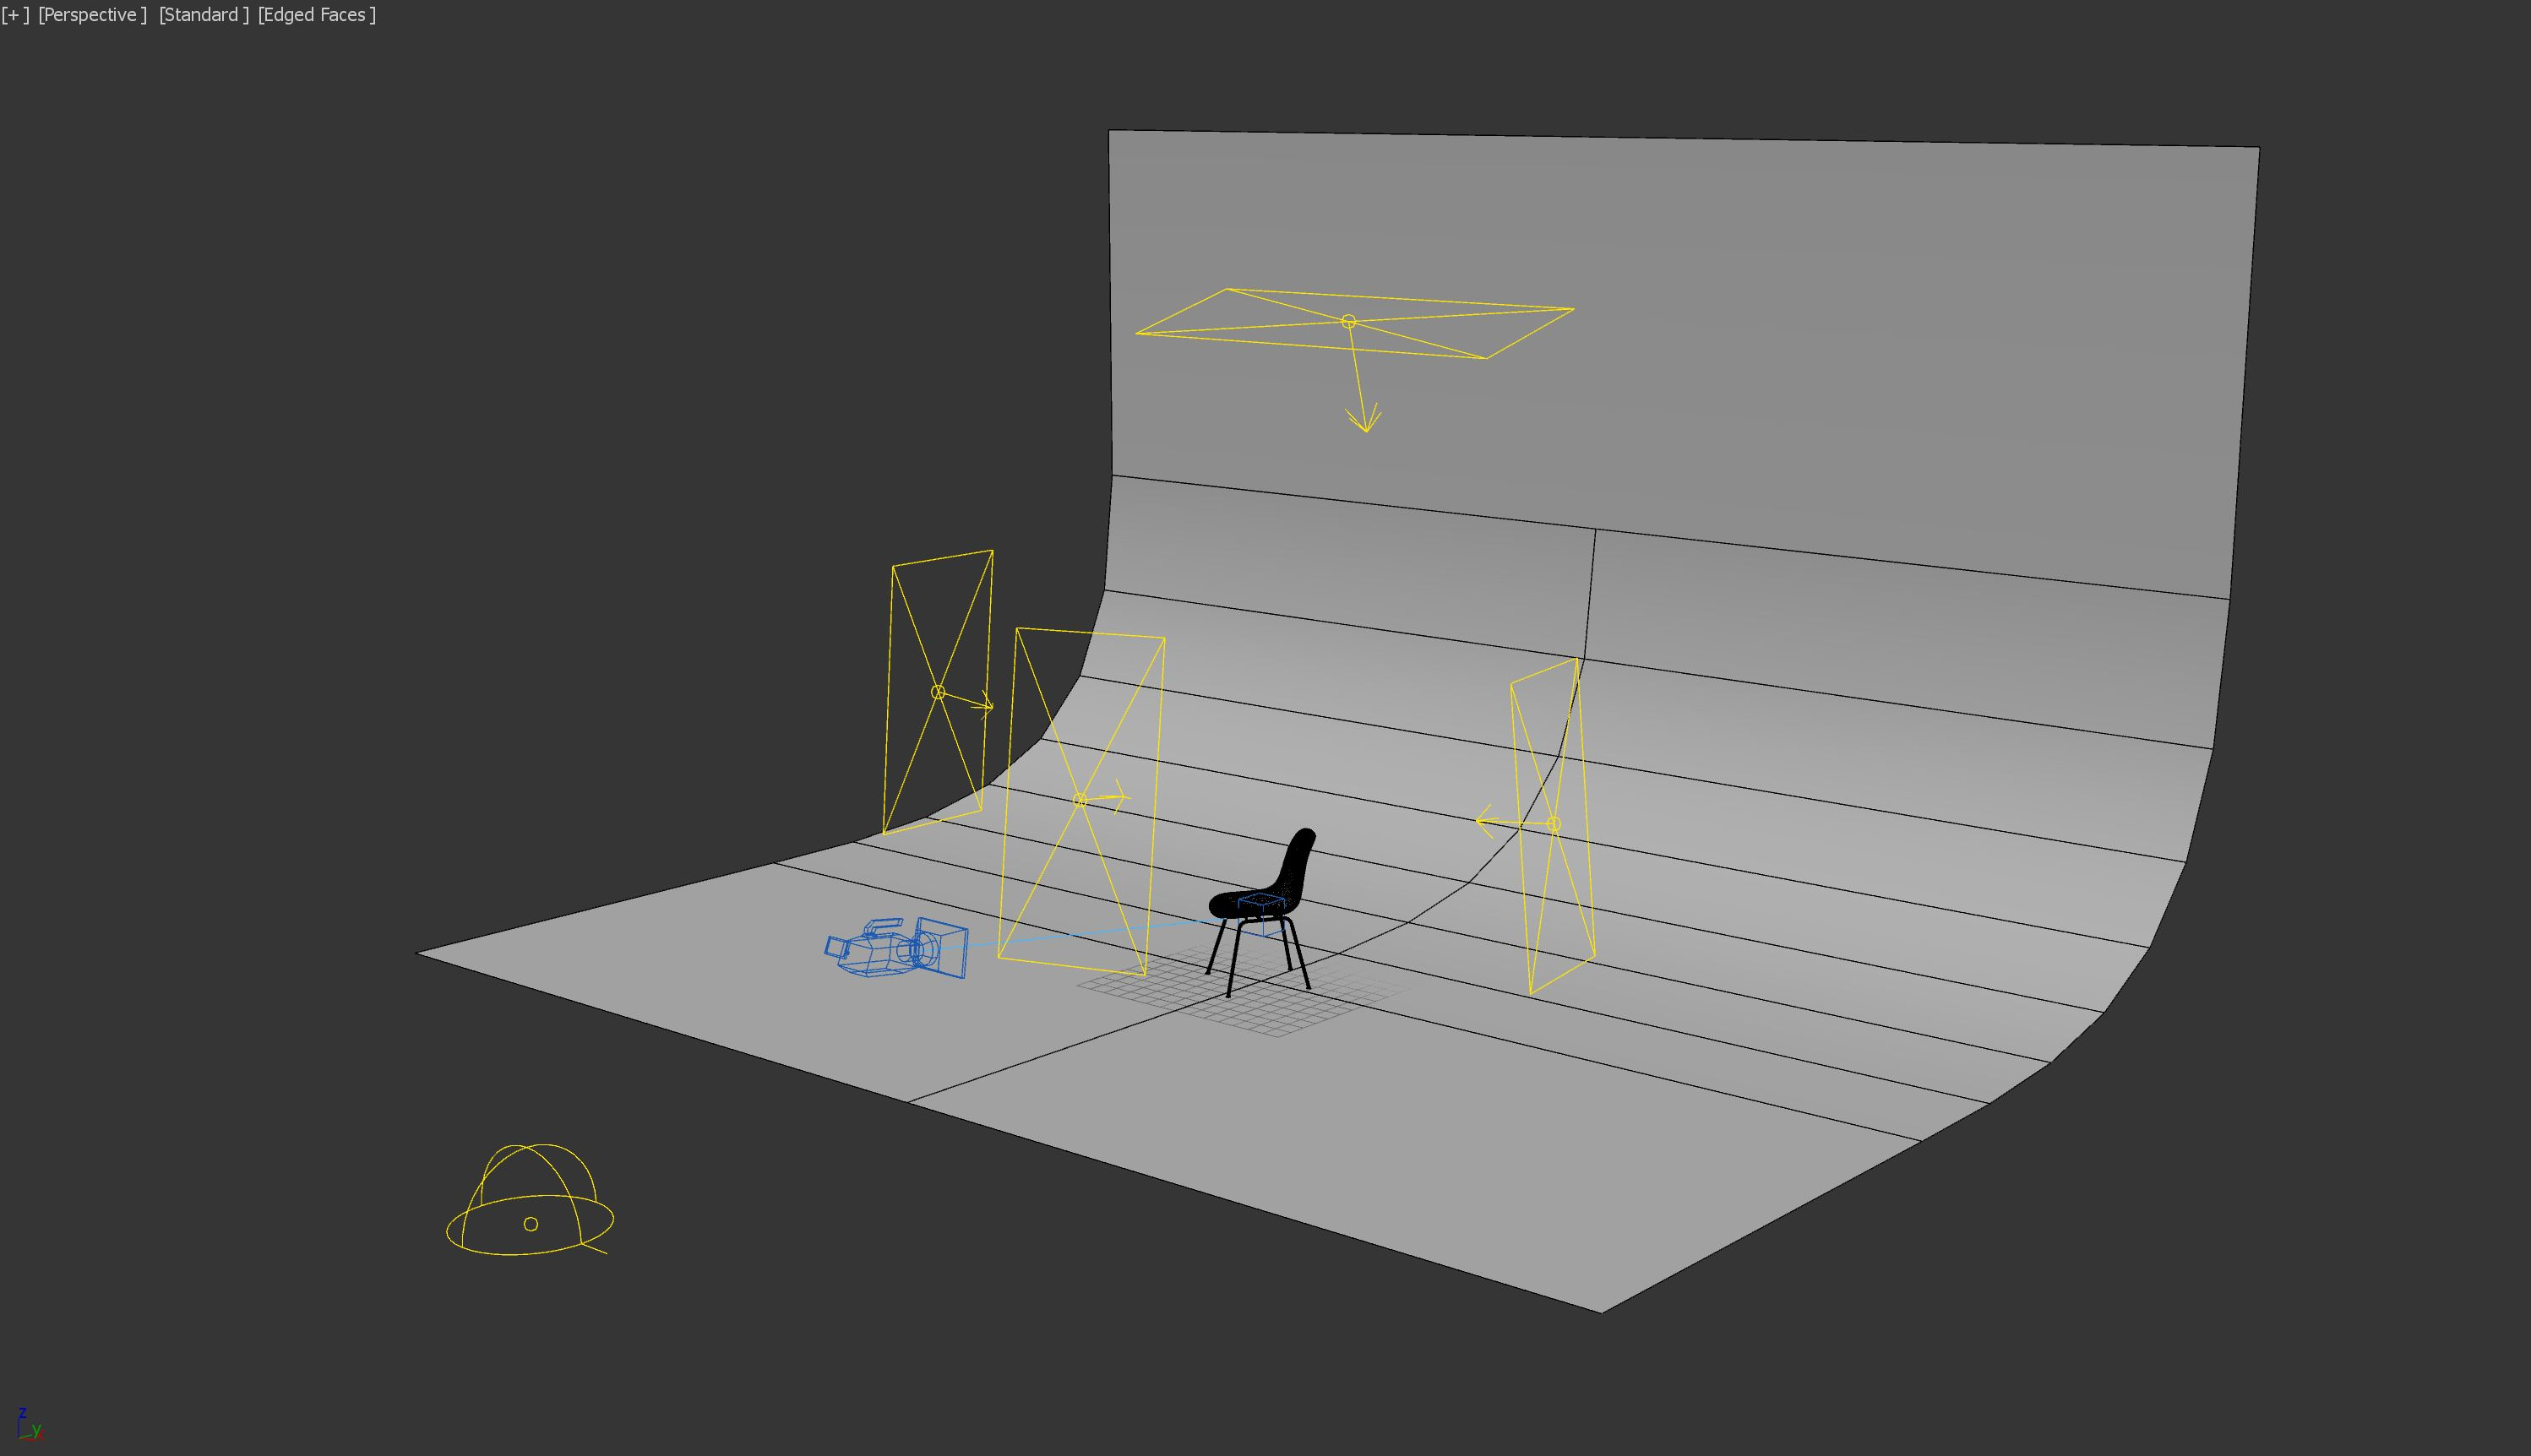
\includegraphics[width=15cm]{images/lighting}
\caption{Lighting Setup}
\label{figure:lighting}
\end{figure}


\subsubsection{Lighting}

\begin{wrapfigure}[12]{r}{10cm}
\vspace{-1cm}
\centering
\includegraphics[width=9cm]{images/lighting_rendered}
\caption{Rendered Lighting Setup}
\label{figure:lighting_rendered}
\end{wrapfigure}

Once in the lighting department, the model is placed into a virtual environment. Most of the time this environment will simulate a photography studio. As seen in figure \ref{figure:lighting}, there are 5 lights in the current setup. One is a dome light that simulates the environment using a so-called 'High Dynamic Range' (HDR) range image. Current .JPG images are 24 bit. As an image is separated into a red, green and blue channel, every colour has 8 bits of information available. This means a jpg image is able to show 256 ($2^8$) shades per colour, so a normal JPG image has $16.777.216$ possible colours in total. \newline
The HDR images are mostly encoded in a 32 bits per pixel option. In laymen terms, this means that an HDR image has more colours per pixel ($4.294.967.296$), than a JPG image has in total. In practice, this means that the extremely bright parts of the image can be used to extract lighting information. The HDR image is mapped onto a spherical dome, which results in the ability to mimic environments without the need for additional lighting. In this case, Peppr used an actual studio environment for that part.
 The other four images are used to light the model to perfection. One on the back to light the background, one in front to have highlights and two diffuse boxes on the side to get the model to stand out from the background.

%----------------------------------------------------------------------------------------
%   Lighting / Shading
%----------------------------------------------------------------------------------------

\subsubsection{Shading}

\begin{wrapfigure}[19]{r}{10cm}
\vspace{-1cm}
\centering
\includegraphics[width=9cm]{images/rendering}
\caption{Rendered image with shaders}
\label{figure:lighting_rendered}
\end{wrapfigure}

Once properly lit, an artist will start shading the model. This is the process of adding life-like materials to the object and making it come to life. This process can be tricky as there are loads of variables involved. Setting the colour is relatively straight-forward. But when it comes to reflections or refractions, things get tricky. Every material reflects in a different way. Not only the amount of reflectivity needs to be set properly, but also the amount the reflections are blurred. Next to that, materials more often than not reflect differently when observed from different angles. These values are directed by the materials Index Of Refraction (IOR \cite{refractiveIndex}, more on that in the render section (\ref{sec:render})). The Index Of Refraction is combined with Fresnel equations (\cite{fresnelEquations}) for a proper reflectivity per angle. The same thing counts for Refractions.
Another thing highly important when defining materials is the objects texture. There are very little materials that are completely smooth. The plastic in figure \ref{figure:lighting_rendered} has an every so slight texture to it. This adds a tiny bit of extra realism.


%----------------------------------------------------------------------------------------
%   Rendering
%----------------------------------------------------------------------------------------
\subsubsection{Render}
\label{sec:render}
This is where things get together and the calculation from 3d model to actual image start. There are two sides to this, the technical settings of the render-engine used and the structure of the file / timeline.
\newline
\textit{Render-engine}
\newline
Peppr opts to use third party render-engines for their projects, mostly due to the speed and quality optimizations. While more configurable, they are also more difficult to use. Many times, there is an equilibrium between quality and render-times. The high render-times have to do with the difficult nature of lights, reflections, refractions and the anti-aliasing of the image. Light for instance, obeys the 'inverse square law' (\cite{inverseLightLaw}), this means the intensity of light decays the further it gets from the point-of-origin. With one light this is quite easy, but imagine having 3 or 10 lights interacting at different intensities from different point-of-views. On top of that, light bounces around. The render-engine will calculate the point of impact, check the properties of the materials it hits and radiate the light back from the surface. The directionality of these light reflections is where things get tricky. The more straightforward the reflections, the easier. A mirror will reflect the light at the same angle of incidence, but when the material is rough, the rays get scattered. For this, the render-engine will sent out multiple rays (for example 50), up to a predefined amount of times. In practice, this may mean that when one ray bounces on a rough surface, it spawns 50 new rays. If all of those rays bounce off of a rough surface again, the rays will amount to 50 x 50. With every bounce, this will increase exponentially.

Refractions makes these things even more tricky because of the Index of Refraction. This specifies change of angle in the lights ray when it goes from one material to another (\cite{refractiveIndex}). Water (at 20c) for instance, has an IOR of 1.333 (\cite{waterIOR}). This means that next to the light rays bouncing, they can also change direction.

The third and last part that makes rendering images a painstakingly long task is anti-aliasing. Anti-aliasing is a way of making the images 'smooth'. It has to do with the square nature of pixels. A diagonal line will not look smooth if it is just one line of pixels. Instead, the pixels directly surrounding it get a semi-translucent fill, which makes the line look smooth. The blending of colours (while not overdoing it) is the anti-aliasing part.

Peppr uses these intricate render-engines to fine-tune the render-settings. For studio setups, where direct lights are the most important light sources, Peppr might choose to use a set of settings where the secondary bounces of light are of lesser quality than for instance an interior, where most light comes from the light bouncing on the floor (mostly indirect).
\newline
\newline
\textit{Automation}
\newline
Sometimes it is easier to render out the whole sequence with every configuration. Other times, it is easier to render just one point-of-view at a time. In the case of the shirt configurator, every shirt had loads of different collars, sleeves, buttons, but also colours. There are numerous ways of splitting this up, automating the process as much as possible. Most 3d applications allow for animations. By changing one aspect of the model for every rendered frame and rending it out as an image sequence, the rendering process can be automated (a bit). The problem with this is that it will always be a choice of lesser evils. While rendering the sequence, it is important to have the most changes possible rendered at once. In the shirt configurator case, this meant splitting it up so that there is a file for every colour. In that way, the file structure is somewhat logical (a file for every colour) and changing one aspect is relatively easy (changing it once, and applying it to the 25 different colours). Unfortunately, this is by no means ideal. Some changes have to be done 25 times (one for every colour).


%----------------------------------------------------------------------------------------
%   Post Production
%----------------------------------------------------------------------------------------
\begin{figure}

\subsubsection{Post Production}
Every 3d model needs a bit of post production. One of the reasons is simply to make the image look better using colour corrections. Another is when the model has layers rendered as masks. This is the step where the images would be split into the different layers. In case of the shirt configurator, this has partly been automated. Using the same animation principles highlighted in the 'Render' section, Peppr made sure they would have one file per colour so they could easily copy changes from one set of colours to another. In the case figure \ref{figure:post_production}, the background has been removed and some slight colour corrections have been made to make the colour stand out a bit more.
\newline
\centering
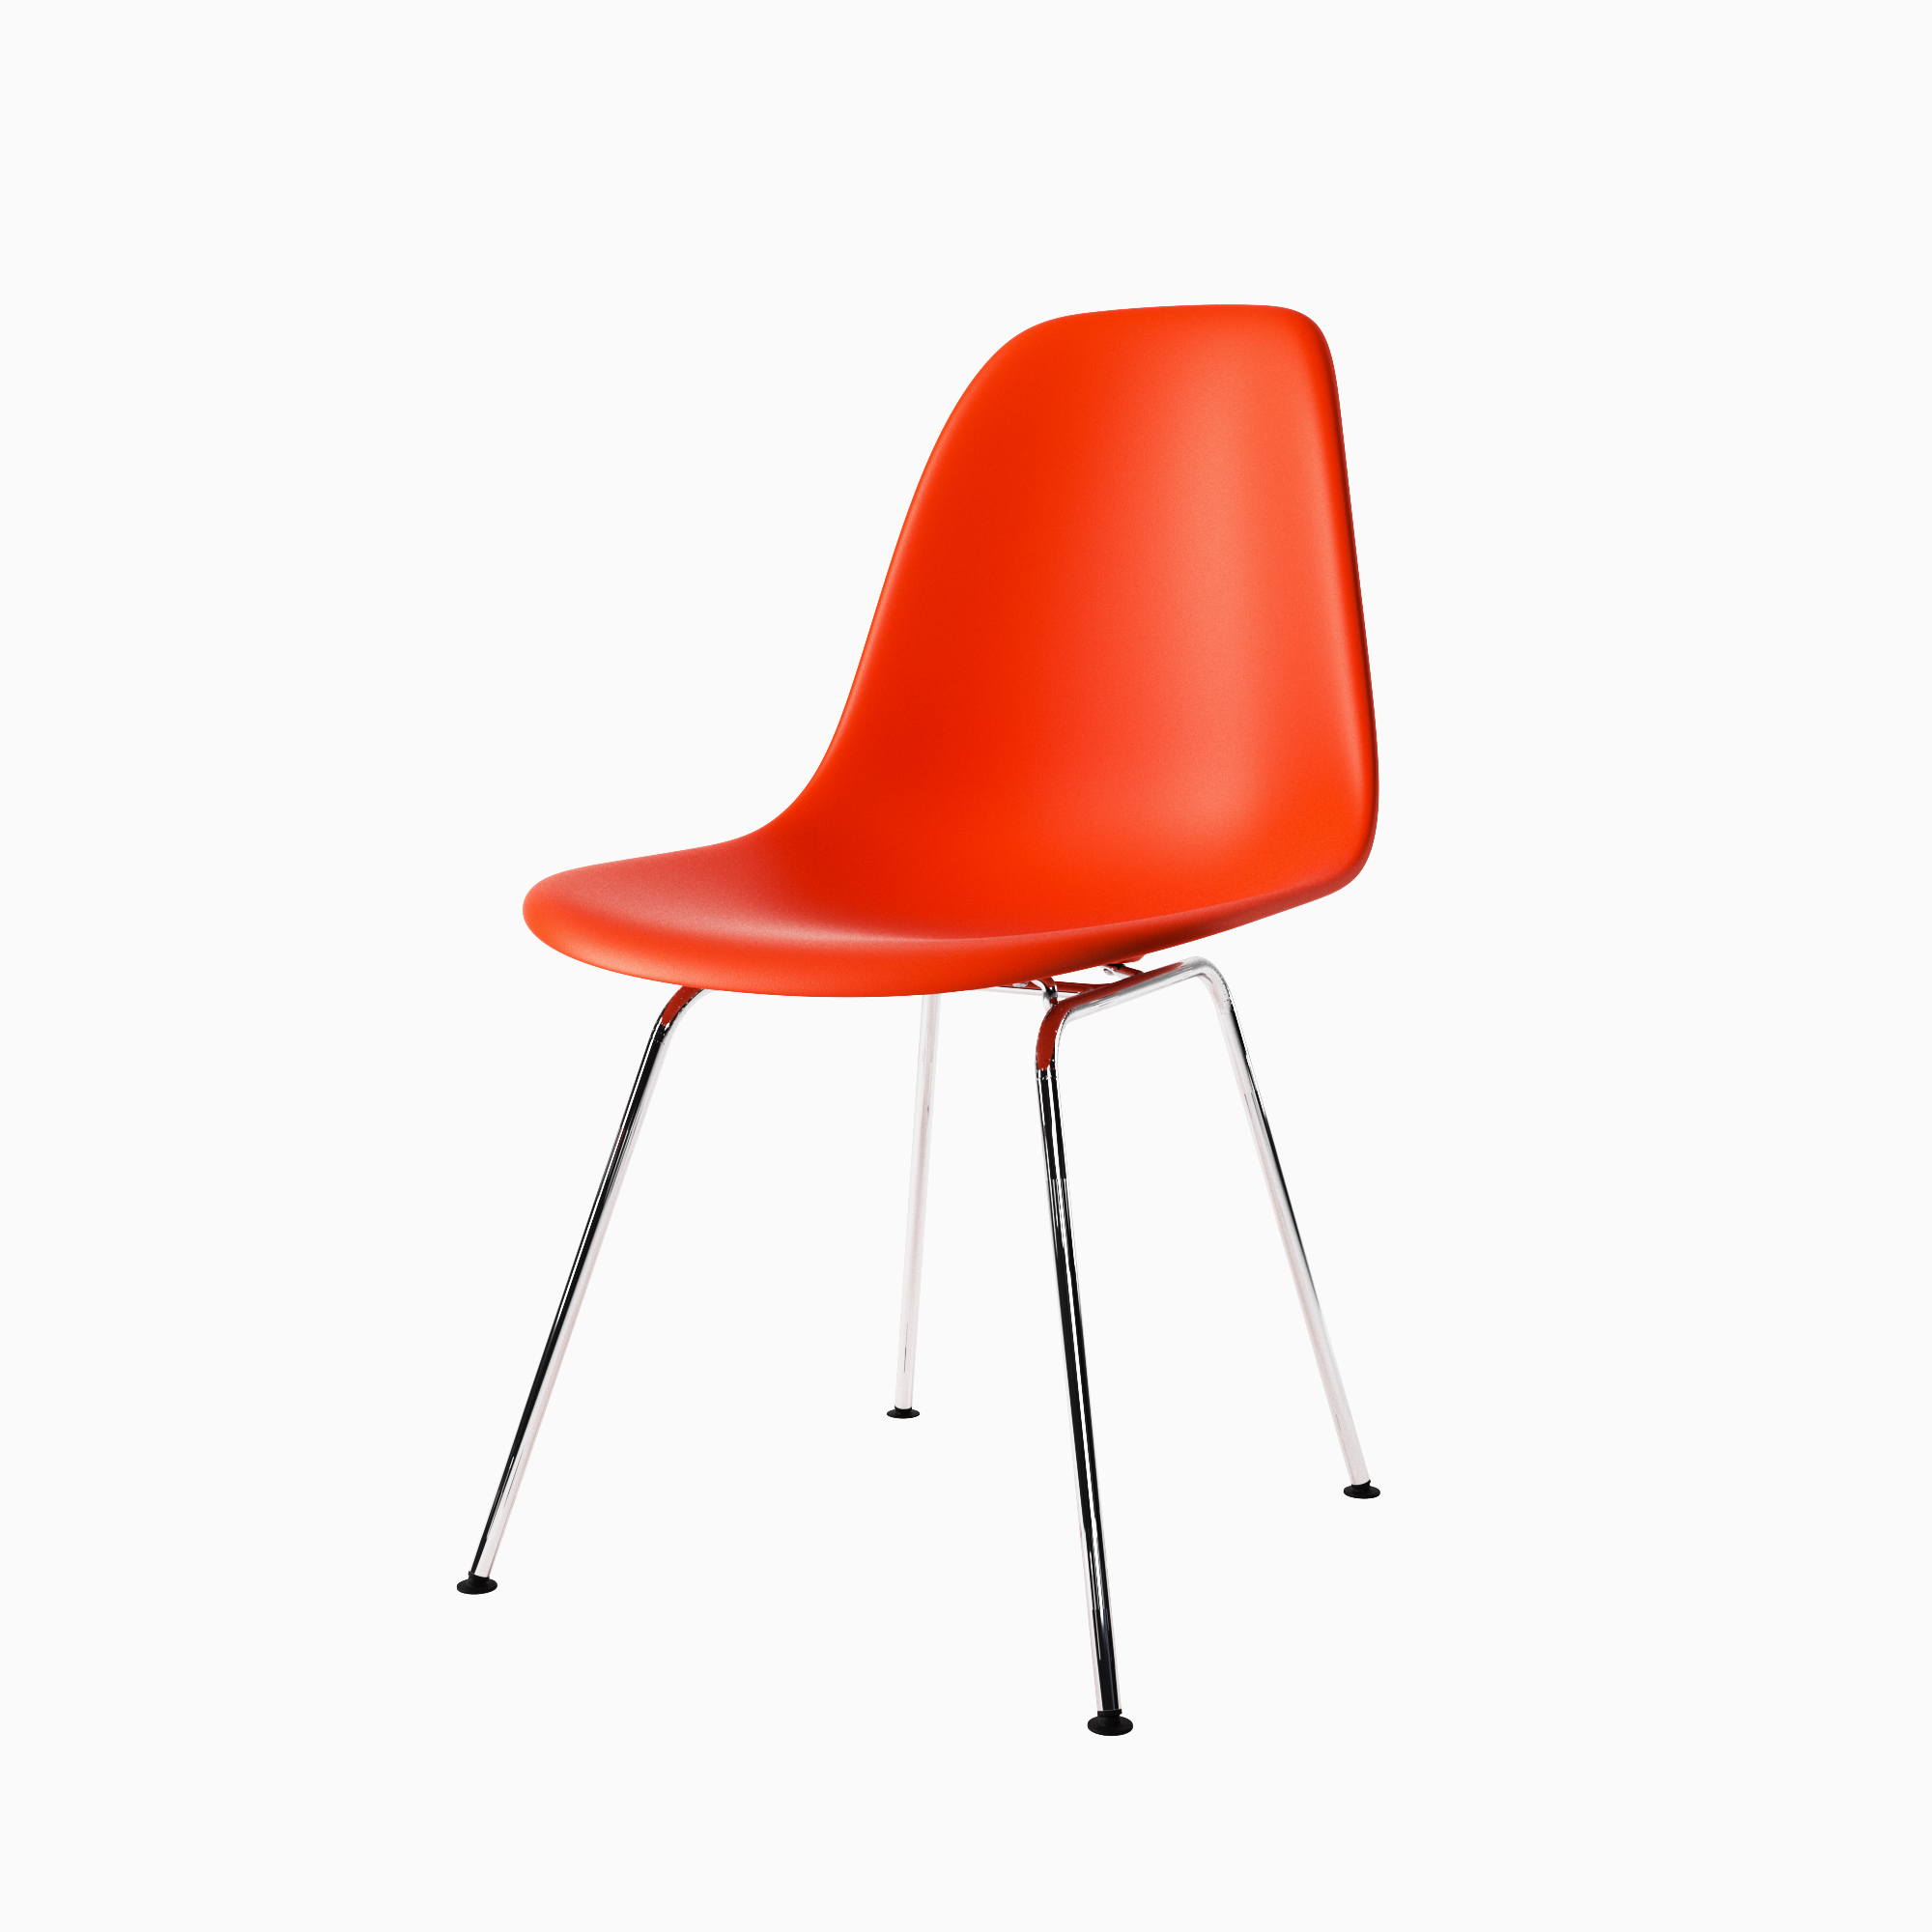
\includegraphics[width=15cm]{images/post}
\caption{The final rendered image with post-production}
\label{figure:post_production}
\end{figure}
%----------------------------------------------------------------------------------------
%   Compression
%----------------------------------------------------------------------------------------
\subsubsection{Compression}
Using images on the web, especially on bigger resolution displays, small file sizes are important. Current mobile data speeds and capped contracts are difficult. So laying a 50mb burden upon the user when opening a site is not a good idea. According to the W3C guidelines, the file size should not exceed 20 kilobytes (\cite{pageFileSizeLimit}). This is were compression comes in. Every images gets compressed for a fast download, while remaining of good quality. The 20kb's stated by the W3C guidelines are unfortunately out-of-question, but a best effort to make the images as tiny as possible is still required.
A couple of things can be done to do this. First and foremost, the image should be the proper size. The rendered image is 2000 x 2000 pixels (w x h). The images for the shirt configurator by Peppr were only required to be 800 x 500. Making the image 800 x 800 reduced it from 445kb to 91kb. This is a massive save in itself, but with proper compression, this can be taken even further. Using an application like ImageOptim (\cite{imageOptim}) , the size is further reduced to a mere 68kb. This in itself is not much, but when there is an image set of hundreds, shaving 25\% off of the filesize counts.


%----------------------------------------------------------------------------------------
%   Aims
%----------------------------------------------------------------------------------------
\subsubsection{Research aims}
\begin{enumerate}
	\item {Is it possible to eliminate all issues with regards to rendering?}
	\item {How easy is it to add new options to the configurator compared to the existing configurators?}
\end{enumerate}

%----------------------------------------------------------------------------------------
%   Software
%----------------------------------------------------------------------------------------
\subsection{Software}
Now that the graphics process has been described. It is time to deep dive into the software development cycle. Mostly, the software and graphics development happen simultaneously with software and graphics working in tandem to make sure they work with each other properly when finished.
​
%----------------------------------------------------------------------------------------
%   Functional Requirements
%----------------------------------------------------------------------------------------
\subsubsection{Functional Requirements}
Functional requirements help map out required functionality of an application. In an agile (\cite{agileUserStories}) working environment, these are 'user stories'. Peppr prefers the term requirements. They do generally use the same notation. \newline

\say{\textit{As a <type of user>, I want <some goal>, so that <some reason>}}\newline

In the context of the configurator specified above, a requirement could be: \newline

\say{\textit{As a \textbf{User}, I want \textbf{to be able to save my configuration}, so that \textbf{I can later continue were I left off with my configuration}}}\newline

%----------------------------------------------------------------------------------------
%   Technical Requirements
%----------------------------------------------------------------------------------------
\subsubsection{Technical Requirements}
Contrary to popular belief, these requirements are not the implementation details of the functional requirements. They are the requirements the system itself. The technical requirements handle things like performance, availability and security. Some put these in a list \cite{agileTechnicalRequirements}, but Peppr uses the same format as the user stories. \newline

\say{\textit{As a <type of \textbf{system}>, I want <some goal>, so that <some reason>}}\newline

Peppr uses this to differentiate between different types of systems. An example of a technical requirement can be found below. This specific one has to do with limiting an API's response time (\cite{responseTimes}).

\say{\textit{As an \textbf{API}, I want \textbf{to respond within 300ms}, so that \textbf{the user feels in control of the application at all times}}}\newline

%----------------------------------------------------------------------------------------
%   CMS
%----------------------------------------------------------------------------------------
\subsubsection{CMS}
A content management system has basic functionality built in (like user management, file handling). It does however, require  the developer to work in the way the system intended. The other option is to go with a system that is written from the ground up. It will be much leaner and quicker when deployed, but will not be as mature as a popular CMS. So if the system is not built right, it may result in a buggy experience for the end user. In Peppr's case, a CMS called Magento was used during implementation. One thing to keep in mind; In case of a custom application, a back-end needs to be developed as well.
%----------------------------------------------------------------------------------------
%   UX Development
%----------------------------------------------------------------------------------------
\subsubsection{UX Development}
While this term gets thrown around a lot, the UX (User Experience) covers not only the UI of the application. It is a broader term to describe how users undergo the experience of customising a product. It is how they learn to use the product configurator. How the application can help the user in the best possible way to do so. Don Normal (\cite{userExperience}) says: \newline
\say{\textit{The first requirement for an exemplary user experience is to meet the exact needs of the customer, without fuss or bother. Next comes simplicity and elegance that produce products that are a joy to own, a joy to use. True user experience goes far beyond giving customers what they say they want, or providing checklist features.}} \newline
In other words, UX is not only helping the user to meet his or her goal. It is to go beyond that, and make the experience joyful.

%----------------------------------------------------------------------------------------
%   Back-End Development
%----------------------------------------------------------------------------------------
\subsubsection{Back-End Development}
Techopedia (\cite{backendDevDefinition}) states that a back-end developer's task is to develop and maintain a logical or computational back-end for a website. Focussing on C++, C\#, Java, or another high-level programming language.Another Definition (\cite{backendDevDefinition}) states back-ends are mostly developed using either Ruby or Python.
In reality, any programming languages that can interact with a databases can act as a back-end. For instance, the 'Dollar Shave Club' uses 6 languages in their infrastructure (\cite{dollarShaveClubBackEnd}). 'Uber', uses a completely different stack (\cite{uberBackEnd}).
Peppr generally uses a microservices architecture for their apps (\cite{microservices}). This pattern allows the use of different applications. So, Peppr can build each application using a specific language and with a specific target in mind. So imagine a configurator needs to stack images but also needs a realtime chatbot. Peppr will be able to handle the high concurrency using something like Elixr (\cite{elixr}) . The realtime chatbot will then made with Firebase, a realtime service (\cite{firebase}).

%----------------------------------------------------------------------------------------
%   Front-End Development
%----------------------------------------------------------------------------------------
\subsubsection{Front-End Development}
According to Wikipedia, a Front-End Developer (\cite{frontEndDevDefinition}) produces the client-side interface. Wikipedia states that they use HTML, CSS and Javascript. However, anno 2016, Front-End Development has become quite a bit broader (\cite{javascriptAnno2016}). For relatively complex projects like configurators, building a front-end can be a daunting task. More often than not, you will want to serve the changes to the user instantly, without a page refresh. Resulting in an asynchronous application.
Building an asynchronous application can be done in many ways. The most convenient way is to build a Single-Page-Application (SPA). This gives the user a desktop-like experience (\cite{singlePageApplications}). As stated on Wikipedia, there are some caveats to this, like search engine optimisation, speed and browser history. Fortunately (and unfortunately), there are frameworks to help build an SPA. Anno 2016, the field of Front-End Development is clouded with frameworks to help build these types of applications. MeteorJS, React, Angular, Vue and many more (\cite{frontEndJavascriptFrameworks} ).
Peppr develops most of their applications using Angular. They found that the code is easiest to maintain and the separation of concerns using a MVC type setup works well with Angular.

%----------------------------------------------------------------------------------------
%   Aims
%----------------------------------------------------------------------------------------
\subsubsection{Research aims}
\begin{enumerate}
	\item {What are the differences in Workflows (both software and hardware)}
	\item {Is the end-result flexible enough to be re-used for other clients?}
	\item {Is the new technology small enough?}
	\item {Is the new technology quick enough?}
\end{enumerate}


%----------------------------------------------------------------------------------------
%   OpenGL & WegGL
%----------------------------------------------------------------------------------------
\clearpage
\section{OpenGL \& WebGL}
Peppr stated the technology that possibly holds the answer is OpenGL and its web counterpart; WebGL.
The first version of OpenGL was released March 2011 (\cite{openGLsite}). It is a software interface to allow programmers to interact with graphics hardware (\cite{openGLSpecification}). It is essentially an API acting as a middle man between software and hardware. In practice, this means that programmers will need only little (to no) hardware knowledge wile still being able to tap into the hardwares calculation capacity. Normally, starting up an OpenGL application, it creates a window that ties into the framebuffer (\cite{framebuffer}), basically a piece of RAM memory containing the bitmap. The application then holds a GL context, and the OpenGL commands can be used to modify and interact with the contents.

To use OpenGL on the web, one needs an API that interacts with OpenGL. This can be done server-side, with the result of the graphics hardware framebuffer being sent to the user (\cite{CRRS}). This means that any language parse-able on a server that can send data out (and has an OpenGL enabled graphics card), can be used. Even though this article stems from 2008, the problems stated with latency still exist today, even while considering their suggested and tested optimisations. Next to that, servers that have graphics cards are relatively expensive. Another option is client-side rendering. With the increase in speed for customer technology and the rise of smartphone usage, the amount of devices that has a graphics card and can use this technology increases. Unfortunately, it is not possible for (most) webbrowsers to directly communicate with the OpenGL framebuffer. Fortunately, there is a solution; WebGL.

\say{WebGL is a cross-platform, royalty-free web standard for a low-level 3D graphics API based on OpenGL ES 2.0, exposed through the HTML5 Canvas element as Document Object Model interfaces.}
\cite{webGL}

WebGL technology renders from the graphics hardware (just like OpenGL). The key difference is that the API is exposed to an HTML5 canvas element. This means the framebuffer is not opened into an application window, but into an HTML5 canvas element. While this solves the issue of running GL content client-side, GLSL (the language used to interact with WebGL \& OpenGL) does not make it into the Stack Overflows Annual Survey (\cite{stackoverflowDeveloperSurvey}). This does imply it would be hard (and expensive) to find competent developers that can built an application using this technology.
Fortunately, Peppr found a library for this. It uses the most popular language in the survey (Javascript). "Three.js", as the library is called, filled the last gap in client-side OpenGL / WebGL content. The question remains, while javascript is adopted in most modern browsers (\cite{javascriptSupport}), will it work in the by Peppr required context?

%----------------------------------------------------------------------------------------
%   Aims
%----------------------------------------------------------------------------------------
\subsubsection{Research aims}
\begin{enumerate}
	\item {Is the technology compatible with the users browsing preferences?}
	\item {What is the development cost difference both in time and money? \textit{While the technology uses a Javascript wrapper, it might not mean that any javascript developer will know how to work with it. Next to that, for a site or Vanilla Javascript application, development cycles and workflows are known. It might mean that reinventing the wheel for these sort of applications because of the use of WebGL might lead to more development time.}}
	\item {How easy is it to maintain the application compared to existing configurators? \textit{For current web technology, a lot has been done to make it easy to maintain (package managers, dedicated servers), but going with a proprietary system that uses OpenGL via WebGL via a Javascript wrapper, might mean that some of these existing solutions will not work. This might mean that the application will be very hard to maintain}}
\end{enumerate}


\newpage







%----------------------------------------------------------------------------------------
%   Aims
%----------------------------------------------------------------------------------------
\include{Aims/Aims}

%----------------------------------------------------------------------------------------
%   Methodology
%----------------------------------------------------------------------------------------



%----------------------------------------------------------------------------------------
%  Introduction
%----------------------------------------------------------------------------------------
\chapter{Methodology}
\section{Introduction}
Developing a product configurator is by any means no easy feat. Building it using 3d technology may be even harder. When doing a small documentary analysis to get and set a proper theoretical framework, it became abundantly clear that there is a lot of research done into the computer science behind the proposed technology (\cite{openGLsite}, \cite{microservices}, \cite{heteregoneousComputingTechniques}). Next to that, loads of research has been done into the User Experience side of (web)applications (\cite{nielsonNormanReports}). Unfortunately, the main question that needs to be answered is quite specific and at this intersection of UX and Computer Science, there is little to no prior research. This means that some of the questions outlined below will need to be answered in an experimental way. There are a couple that can only be answered using this experimental type of setting. However, there are also some questions that could be answered using interviews or a documentary analysis. But with the need of actually building a prototype, going that way would be harder than to device an experiment using the prototype.
Basically, all questions that have to do with the development cycle, can be answered using this experimental type of research. Questions regarding the UX mostly will follow a combination of multiple methods (as we need to define certain standards). The start of this section will be a deep dive into the methodology behind building the prototype, followed by the ways of researching the development and user experience research objectives.

%----------------------------------------------------------------------------------------
%   Experimental Prototype
%----------------------------------------------------------------------------------------
\section{Prototype Preparation}
\subsection{Introduction}
To keep the prototype as simple as possible, an analysis of the requirements will be made. After which a development stack shall be chosen and the development will be started. As a rough example, the example used in the theoretical framework shall be used. Most of the workflow in the build of this prototype shall be inherited from Pepprs current Software Workflow.

\say{
A chair manufacturer wants a product configurator for one of their most popular chairs. It has 25 different colour options and has 4 different subframes. Two of the subframes are steel and can be either black or plain. The other two have wooden elements and have four wood colour options.
}

\subsection{Requirements}

\subsection{Functional Requirements}
Looking at the outline above, there are basically two things the configurator needs to do; switch models (for frames) and switch colours (for both frames and chair itself). This should (logically) all be wrapped in a user interface where the user can switch the colours and models with their cursors. Some other things, inherit to product configurators are needed as well. To map these requirements in a way Peppr would do, these would amount to the following;

\begin{itemize}
	\item As an end-user, I want a friendly way to change the colour of the chair
	\item As an end-user, I want a friendly way to change the model of the frame
	\item As an end-user, I want to see my newly build configurator in enough ways to make a proper assertion as to wether or not I would buy this object
\end{itemize}

Dissecting these user-stories, some conclusions can be made as to what the front-end application of the system should do.
\begin{itemize}
	\item As a front-end, I need to be able to load 3d models into my scene
	\item As a front-end, I need a way to switch 3d models
	\item As a front-end, I need a way to have materials on the 3d models
	\item As a front-end, I need to show the 3d model realistic enough so the end-user can make a buy / do not buy choice
	\item As a front-end, I need to have a way for the user to navigate the scene and see the model from several points-of-view
	\item As a front-end, I need a way to know what colours the chair might have, so I can show the user his / her options
	\item As a front-end, I need a way to keep track of what models are in my scene, so I can apply the colour to the right object
	\item As a front-end, I need a way to keep track of the current configuration, so switching between different configurator options will keep the current configuration
\end{itemize}

From here, some user-stories for the back-end can be made.
\begin{itemize}
	\item As a back-end, I need to be able to supply 3d models to the front-end
	\item As a back-end, I need to show the front-end what options are available (both for models, as well as colours)
	\item As a back-end, I need to supply multiple 3d models if any configuration requires more than one model for a subset
\end{itemize}

While always difficult to estimate the exact requirements upfront, building a product configurator prototype using this short set of functional requirements should be sufficient to answer the research questions. 

\subsection{Technical Requirements}
Technical requirements are tricky in this case, as the prototype should be flexible and setting hard demands on for instance load times or uptimes, would interfere with the experiment. The most important thing is to see wether or not the functional requirements can be integrated and at what cost. The question for now is 'if' it is implementable, not when or how. As such, the technical requirements will be left unspecified.

\subsection{Technology Stack}
Now that the requirements are set, the technology stack can be chosen. Below are the three most important components for this stack. The 3d section (\ref{subsub: 3d}) is where is explained if and if so which framework is necessary for the front-end of the application to handle and render the 3d files in realtime. In the front-end section (\ref{subsub: frontEnd}) several front-end setups shall be discussed. An explanation of why there is no need for a back-end in this prototype will be given in the back-end section (\ref{subsub: backEnd})

\subsubsection{3d}
\label{subsub: 3d}
To display and render 3d models in browser, one can directly use the webGL api (\cite{webGL}). However, there are frameworks that make most of the work easier. There are loads of libraries that offer 3d capabilities in browsers, but the two most popular frameworks are ThreeJS (\cite{threejs}) and Babylon (\cite{babylon}). Having little to no experience with these libraries, the decision on which framework to use was made based on the amount of stars on Github. Babylon was starred 4479 times, ThreeJS 32.763 times, making ThreeJS the clear victor. Next to that, there are over 18.000 commits on the ThreeJS and only a bit more than 6.600 on the Babylon Framework.

\subsubsection{Front-end}
\label{subsub: frontEnd}
Apart from the 3d specific side of the front-end, things like styling buttons and setting HTML syntax should be handled as well. Both of these are easily chosen, basic HTML 5 will suffice for the lather, while an SCSS / SASS (\cite{scss}) is used for styling. SCSS has the advantage over CSS in that it has the ability to nest components, and use functions and variables. So in CSS, one would write something like this;

\begin{lstlisting}[language=CSS]
.button {
	background-color: #333;
	border-color: #333;
}
.button:hover {
	background-color: #000;
	border-color: #000;
}
.button.button-success {
	background-color: #00ff00;
	border-color: #00ff00;
}

.button.button-success:hover {
	background-color: #00dd00;
	border-color: #00dd00;
}
\end{lstlisting}

\clearpage
While in SCSS, one would do the following. While it takes up slightly more lines of code, the obvious advantages are readability, but also that one can specify colours and variables in one place and change the look of an entire application with just these variables.

\begin{lstlisting}[language=CSS]
$button-clr: #333;
$button-clr-success: #00ff00;
.button {
	background-color: $button-clr;
	border-color: $button-clr;
	&:hover {
		background-color: darken($button-clr, 10%);
		border-color: darken($button-clr, 10%);
	}
	
	&.button-success {
		background-color: $button-clr-success;
		border-color: $button-clr-success;
		&:hover {
			background-color: lighten($button-clr-success, 10%);
			border-color: lighten($button-clr-success, 10%);
		}
	}
}
\end{lstlisting}

So for displaying the control components, SCSS and HTML 5 will do. For the 3d, ThreeJS will be used. The only component in this stack that is not accounted for, is data and data flow. How does the ThreeJS component know that an HTML 5 button was just pressed? There are loads of ways to handle data flow within an application, MVC, MVP, MVVM (\cite{MVCMVPMVVM}) and loads of Javascript front-end frameworks to choose from (\cite{javascriptAnno2016}). While the lather article explains the state of front-end development quite humorously, there is some truth to this. This means choosing a framework to use is tricky. In case of this prototype Peppr thought it would be best to use that which they are familiar with and have used in a variety of projects; Angular. At the time of writing Angular 2 has just been released out of beta, but support for it with the relatively quick upcoming version of Angular 4 (they skipped version 3) do not make it suitable for building this prototype.
There is a bit of a learning curve to Angular and performance is one of the biggest short-comings. The performance troubles Angular deals with are mostly due to the data binding and DOM watching though. This is something the prototype will not be bottlenecking on. There will be little to no watchers as the frame buffer for the 3d output will be rendered to a Canvas element, in which there are no Angular watchers.

\subsubsection{Back-end}
\label{subsub: backEnd}

%----------------------------------------------------------------------------------------
%   The Prototype
%----------------------------------------------------------------------------------------
\section{The prototype}
\subsection{Introduction}

%----------------------------------------------------------------------------------------
%   Development
%----------------------------------------------------------------------------------------
\section{Development}

%----------------------------------------------------------------------------------------
%   Is it possible to eliminate all issues (time and automation) with regards to rendering?
%----------------------------------------------------------------------------------------
\subsection{Is it possible to eliminate all issues (time and automation) with regards to rendering?}

%----------------------------------------------------------------------------------------
%   What is the cost differences for development?
%----------------------------------------------------------------------------------------
\subsection{What is the cost differences for development?}
% Estimate time for both projects
% Find 3d pricing
% Find developer pricing for CMS
% Find developer pricing for custom
% Check server costs
% Check CMS average upgrade cyclus
% Check NPM package average upgrade cyclus
% Check main NPM package upgrade cyclus
% Initial, Server costs, Upgrade costs

%----------------------------------------------------------------------------------------
%   What are the differences in Workflows
%----------------------------------------------------------------------------------------
\subsection{What are the differences in Workflows?}

%----------------------------------------------------------------------------------------
%   How flexible is the end result compared to previous generation configurators
%----------------------------------------------------------------------------------------
\subsection{How flexible is the end result compared to previous generation configurators}
% Estimate time in old way
% Find 3 different product configurators
% See how far we get re-building them using the CMS
% Estimate time in new way

%----------------------------------------------------------------------------------------
%   How easy is it so maintain the application compared to existing configurators?
%----------------------------------------------------------------------------------------
\subsection{How easy is it so maintain the application compared to existing configurators?}
% Interview Frederick with regards to maintaining the application / costs (what is it like owning a setup like that)
% --> from "What is the cost difference for development?"
% Use CMS average upgrade cyclus
% Use NPM package average upgrade cyclus
% Use main NPM package upgrade cyclus

%----------------------------------------------------------------------------------------
%   How easy is it to add new options to the configurator compared to the existing configurators?
%----------------------------------------------------------------------------------------
\subsection{How easy is it to add new options to the configurator compared to the existing configurators?}
% Estimate time in old way
% Add new options to configurator
% Estimate time in new way

%----------------------------------------------------------------------------------------
%   User Experience
%----------------------------------------------------------------------------------------
\section{User Experience}
Apart from the development cycle, the user experience is a huge part of whether using these types of configurators is viable or not. Even if the development is way cheaper, if users cannot use the application, problems will arise and the old method may prove to be a better option.

%----------------------------------------------------------------------------------------
%   Is the technology compatible with the users browsing preferences?
%----------------------------------------------------------------------------------------
\subsection{Is the technology compatible with the users browsing preferences?}
% Scan 'caniuse.com' for theoretical problems
% Setup domain with browserify and see how it renders

%----------------------------------------------------------------------------------------
%   Is the new technology small enough?
%----------------------------------------------------------------------------------------
\subsection{Is the new technology small enough?}
% Record network activity for three other product configurators that have a comparable setup
% Record network activity for OpenGL version
% Find average site size
% Find psychology behind it

%----------------------------------------------------------------------------------------
%   Is the new technology small enough?
%----------------------------------------------------------------------------------------
\subsection{Is the new technology quick enough?}
% Old -- Record / time switching between 'models'
% Old -- Record / time switching between 'materials'
% New -- Record / time switching between 'models'
% New -- Record / time switching between 'materials'
% Use data from bandwidth to calculate average loading time per network type (2g, 3g, 4g, etc.)

%----------------------------------------------------------------------------------------
%   Results
%----------------------------------------------------------------------------------------
    
    
\chapter{Results}
Here I'll state the findings on the research per domain objectives, with a research conclusion in the end.
	This will contain a go / no go moment, in which shall be decided if the building section shall be finished within this research.
	

\chapter{Discussion}

\chapter{Conclusion}

\chapter{Attachments}

%----------------------------------------------------------------------------------------
%   Abstract
%----------------------------------------------------------------------------------------
\bibliographystyle{apalike2}
\bibliography{Bibliography/bibfile}

\end{document}§